\section{Graph Design}
In the graph design process there are two main areas which require consideration - these are syntatic (\autoref{semantic}) and semantic (\autoref{syntatic}) representation. In this section I will explore the different automated graph layouts which can be used to represent our data (syntatic) and the methods in which we may increase the net amount of useful information presented to the user once the graph layout has completed (semantic). 



\subsection{Graph Syntatics}\label{syntatic}

 Syntactic representation considers how best to distribute the information on the given page for maximum impact. An example of this is seen in \autoref{fig:worldmap}, whereupon the flights between airports are represented using a force-directed graph layout (top), and their geolocation (bottom). 
 The graph provides a clearer representation on the relationships between airports, whilst the geo layout gives a more accurate representation of the distances between unconnected nodes (airports). Decisions on what syntatics best represent the feature of interest are an important part of the visualisation process. 
 
\begin{figure}[H]
     \centering 
      \begin{subfigure}[b,black]{.9\textwidth}
         \centering 
     \includegraphics[width=\textwidth]{figures_c1/layout/layoutforce.png}
     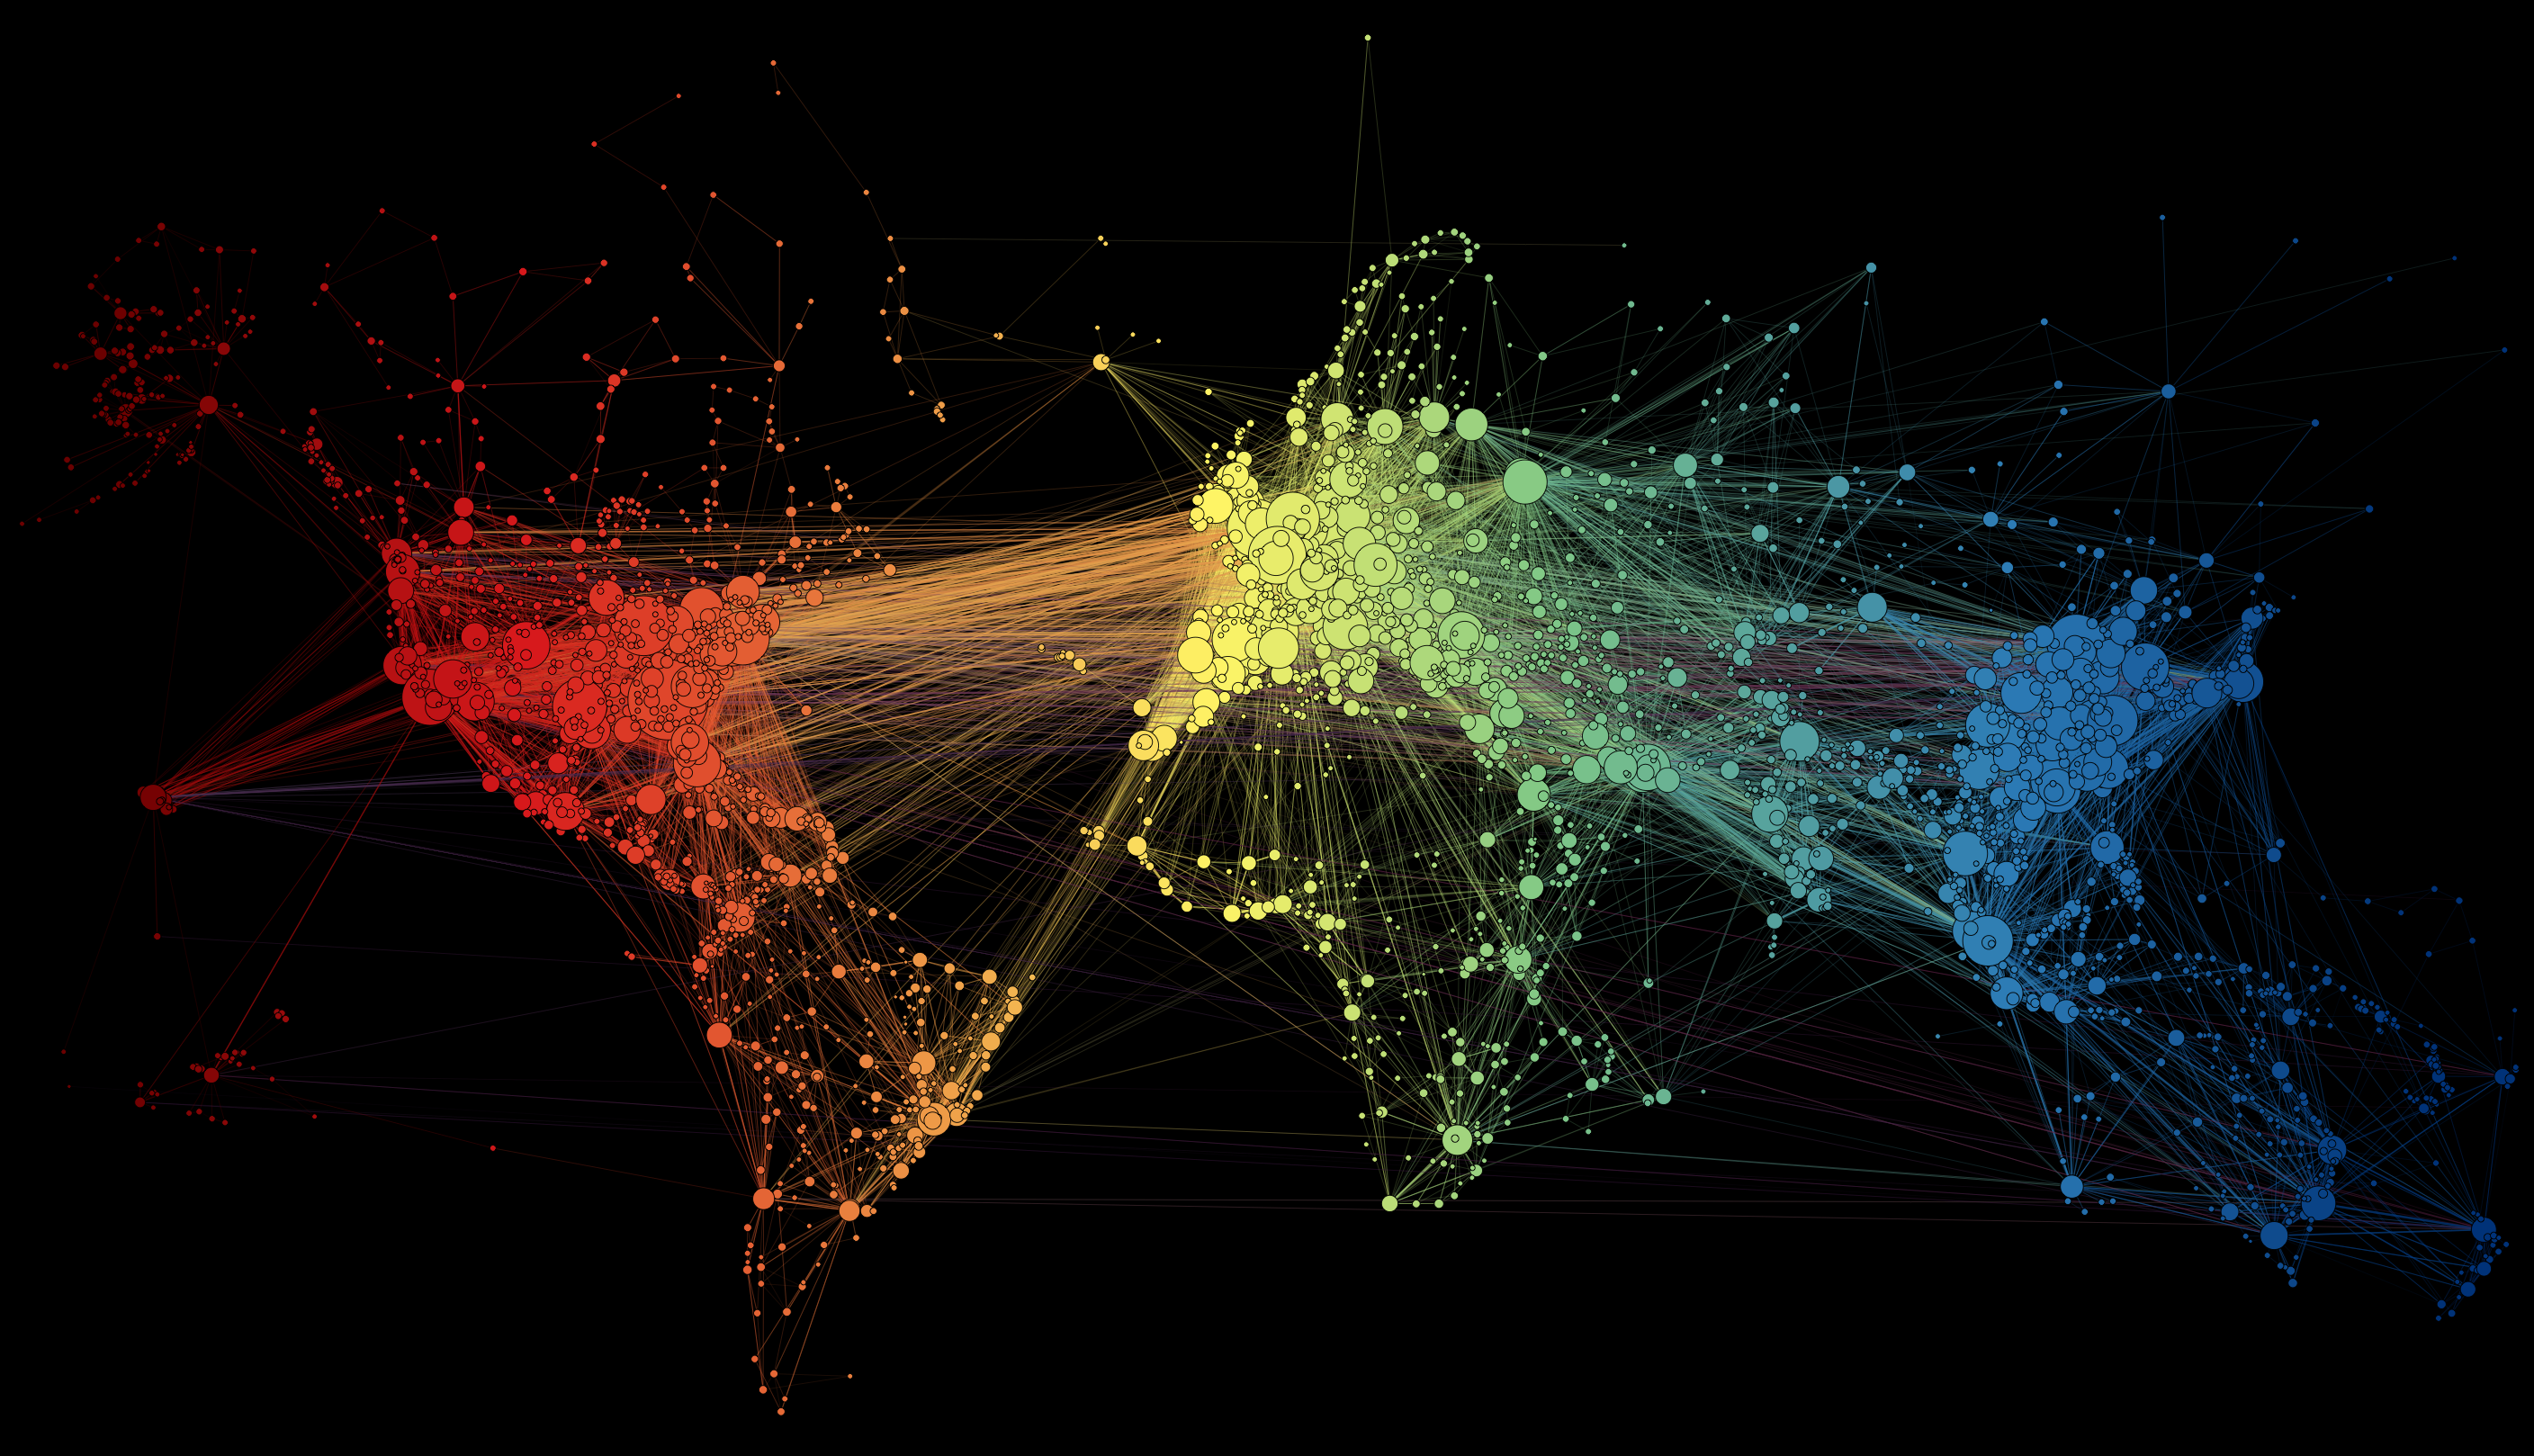
\includegraphics[width=\textwidth]{figures_c1/layout/layoutgeo.png}
     \end{subfigure}
        \caption{\textbf{Comparison of different representations of flight data by \cite{worldmap}.} The top figure shows the data represented by a force directed graph layout (described below) and a Geo-layout showing each point at its location on the Earth.}
        \label{fig:worldmap}
\end{figure}


\subsubsection{Criterion Choices}
Since chemical networks can provide a wealth of information, this can prove challenging to both user cognition and  physical (computational) resources \cite{ch1}.There are many metrics for improving a visualisations aesthetics, \cite{metricgraphaesthetics}, however theseare often evaluated only for a limited number of criterions. This makes it diffucult to accurately quantify the changes in user-readability, especially if these are treated differently than was originally intended, \cite{eyetrack}. 


\paragraph*{Edge Crossing and Bends} \label{edgecross}
One of the greatest limitations to understanding a graph is the number of crossing edges \cite{humanaesthetic}. Experimentation with eye tracking software found that in determing information about the structure of a system users spent more time looking at the edges than the nodes themselves, \cite{eyetrack}. 

Several styles of layout algorithms (e.g. force-directed, orthogonal) aim to reduce these by introducing repulsive forces, or constraining the shape of each edge within the graph. The use of orthogonal designs has been proven for circuit chematics and transport networks, however they lose any information that may be encoded in a nodes relative location. A reduction of the accuracy is also seen in simple tasks where users are required to name the nodes along a chosen path compared to a force directed layout (58/100:92/100), \cite{eyetrack}. Finally the use of bends may be misleading as users can perceive them as multiple separate objects \cite{aestheticsgraphvis}.
    
 
\paragraph*{Node Distribution}
Having nodes equally distributed across the visualisation area can also increase the readablity of a grap. In addition to preventing overlapping edges, equally distributed networks with medium lengh edges greatly improves the `flow' of the diagram. Coupling this with graphical-symmetry is seen as the next most important user-ranked preference, \cite{ch6graphredability}. 


\paragraph*{Node Overlap}
As with overlapping edges, if two nodes are positioned in the same point in space it makes it difficult to read a graph. Historically many algorithms treat nodes as point masses which would makes it dificult of designers to remove the overlap betwen them \cite{nodeoverlap}.

To remove any node overlap there are two main methods, \cite{IPSEPCOLA}. These are:

\begin{itemize}
\item [1.] Create a layout design capable of taking node size (e.g., \cite{nons}) into concideration. These designs tend to be layout specific and not absolute in removing all overlap between nodes. 
\item [2.] This requires a level of post processing in the form of a `layout adjustment'. Here we reposition nodes after a chosen layout has finished computing. The drawback of this method is that information contained in the graph's shape may be degraded. This can be done through the use of collision detection, or moving nodes to the centre of the vernouli cells \cite{novern}. 
\end{itemize}


% \paragraph*{Chosen Criterions and analysis}
% 
% In addition to these, we wish to reduce any regions of high density (inter-conductibility) for large numbers of nodes, since this reduces graph readability, whilst retaining the modular structure of the chemistry due to its nnnn nature. 
% 
% In \autoref{sec:drawing} we explore the distribution of nodes for a network for a range of layouts. Spatial zzzz is determined through the use of $x-y$ kernel density profiles and a density contour plot.
% 



\subsection{Automated Graph Drawing Layouts}\label{sec:drawing}

In their design and evaluation, automatic graph drawing algorithms are created as to minimise a specific criterion. In this subsection I explore several graph drawing algorithms, and juxtapose them to determine which may be best suited for the applictaion to atmospheric chemistry model representation. To do this a MCM subset representative of the APHH Beijing campaign [?ref?] is used. This provides the foundation for a real-world case study which may be simulated in a chemical model. 

\subsubsection{Replication of hand-drawing methods}
With the rise of computation many traditional visualisations were adapted for computer aided generation. Fields of architecture and circuit design adopted computational software to alleviate some of the difficulties presented by large or complex designs. Similar ideas such as the use of automatically generated transit maps  can be used to link chronological or topological items such as ideas, \cite{memory}. \autoref{fig:mem} shows all the possible paths for the oxidation of methane to produce carbon dioxide (and water). Although such methods can be useful in showing isolated path ways, they provide a convoluted representation of large interconnected systems and require some manual intervention. 



\begin{figure}[H]
     \centering
     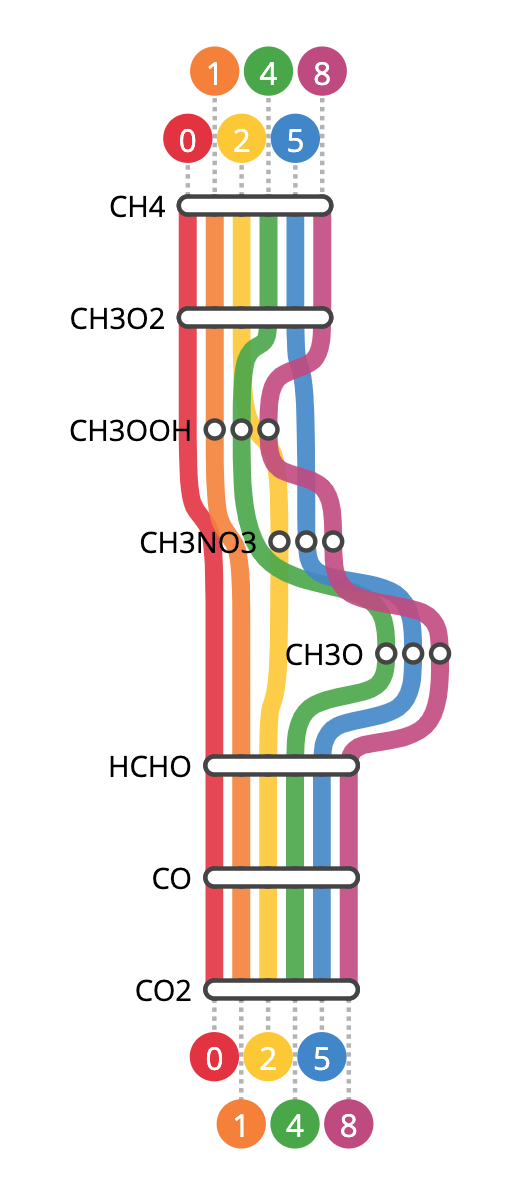
\includegraphics[width=0.25\textwidth]{figures_c1/layout/memory.png}
         \caption{\textbf{A transit map showing all the possible routes from methane to carbon dioxide.} This was drawn using MemoryMap (\cite{memory}) and uses a version of the MCM methane subset, where carbon dioxide has been introduced. }
        \label{fig:mem}
\end{figure}





\subsubsection{Projection Based}\label{sec:merc}
One of the oldest fields of data visualisation fall in the realm of cartography. Here the shapes and distances between points on the surface of the earth (an oblate spheroid) are mathematically mapped onto a 1D plane for graphing purposes \cite{projections}. Since the process of dimensionality reduction will produce inherent distortions within the final product, we end up with a range of map projections, with each striving to achieve a different aim, \autoref{fig:projections}. The Pierce Quincucial for example is a conformal mapping technique mapping the surface of a sphere to a square with very little deviation in scale and the ability to be tessellated in all directions. The Mercator  on the other hand is a cylindrical projection which grew in popularity due to its unique ability to represent any course of constant bearing\footnote{Also known as a `rhumb`, or `loxodrome`, and consists of an arc crossing all meridians of longitude at the same angle.} as a linear segment within the shipping and navigation industry. 

\begin{figure}[H]
     \centering
      \begin{subfigure}[b]{.25\textwidth}
         \centering
     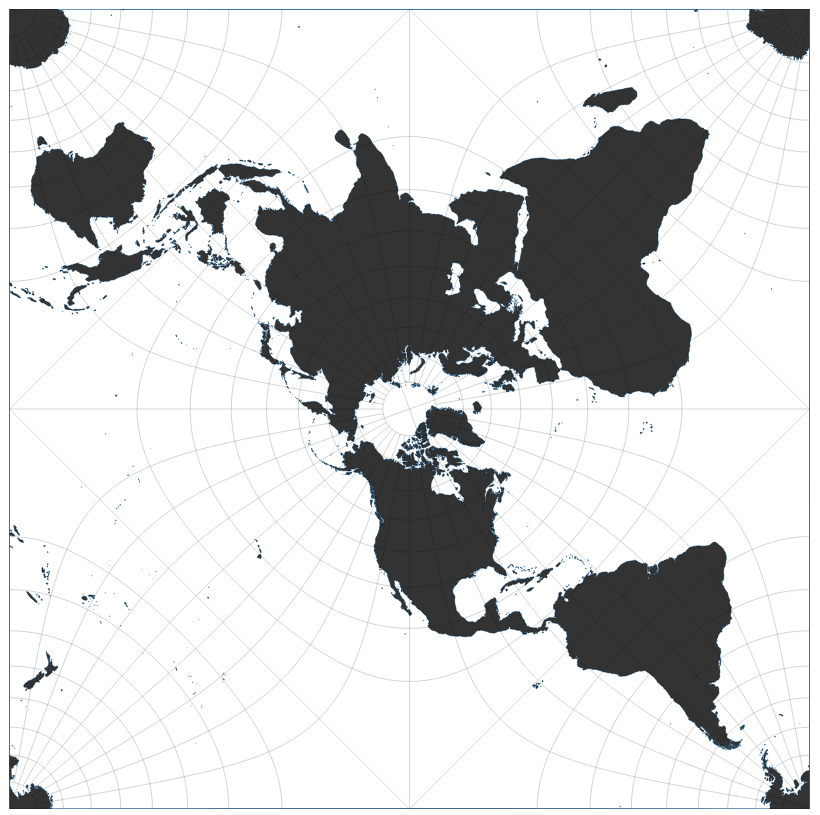
\includegraphics[width=\textwidth]{figures_c1/layout/pierce.png} \caption{Pierce Quincucial}
     \end{subfigure}
    \begin{subfigure}[b]{.3\textwidth}
         \centering
     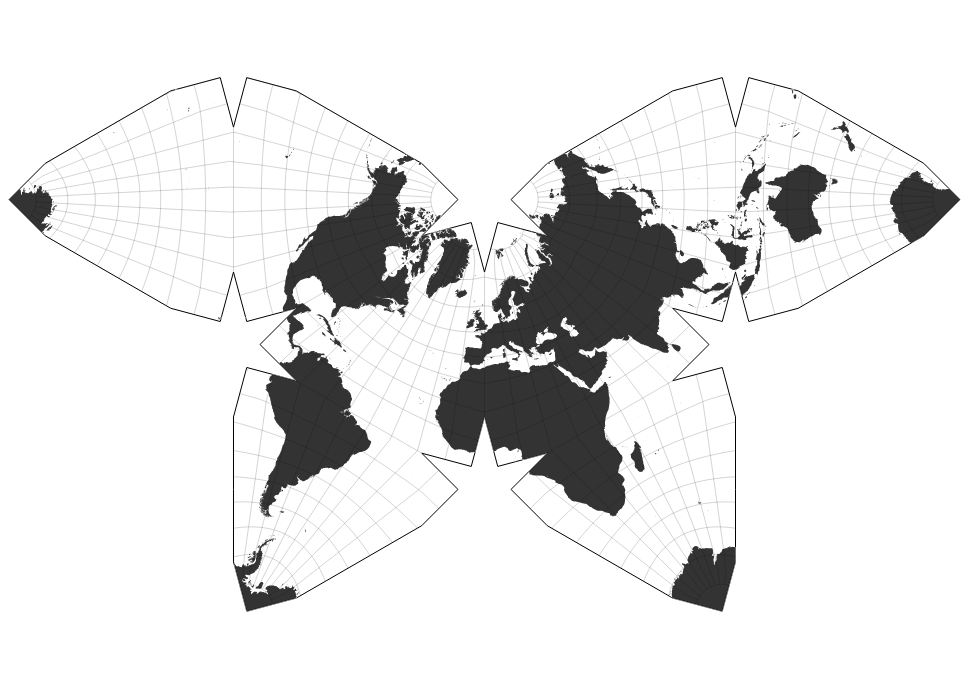
\includegraphics[width=\textwidth]{figures_c1/layout/waterman_butterfly.png}
     \caption{Waterman Butterfly}
     \end{subfigure}
     \begin{subfigure}[b]{.3\textwidth}
         \centering
     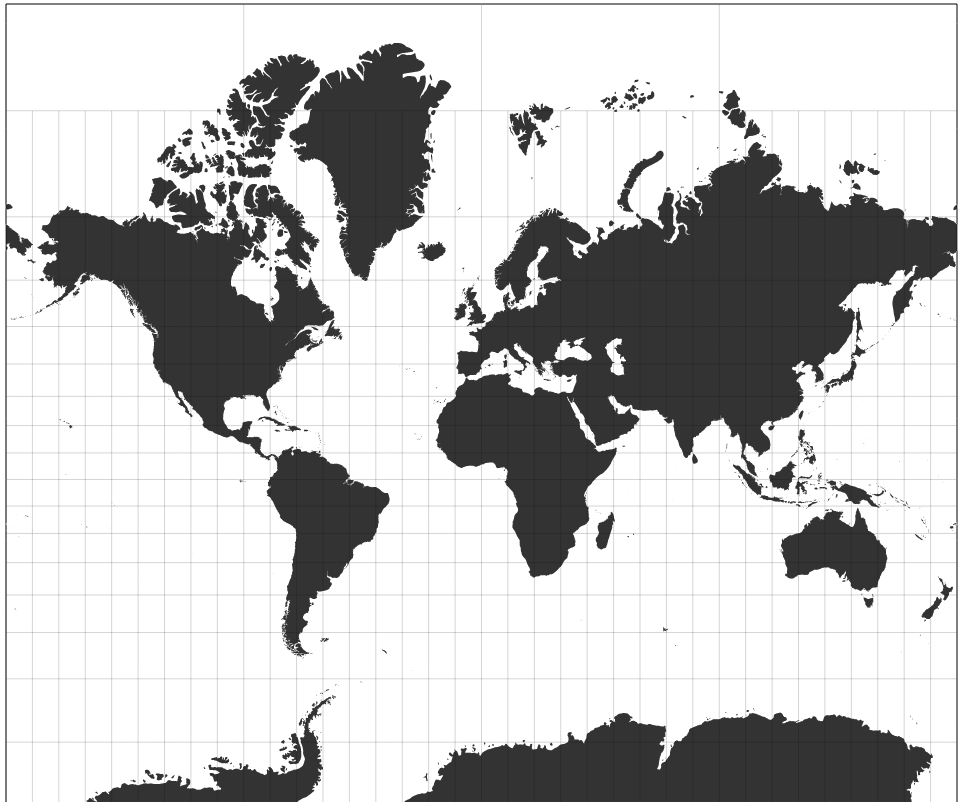
\includegraphics[width=\textwidth]{figures_c1/layout/mercator.png}
     \caption{Mercator}
     \end{subfigure}
        \caption{\textbf{A selection of map projections.} These have been created using DataDrivenDocuments (\cite{d3}) and show a range of methods for mapping the spheroid shape of the Earth onto a 2D plane. }
      \label{fig:projections}
\end{figure}

More recently, the mathematics of mapping a large dimension onto a simpler one have been applied to the problem of graph representation. \cite{mercgraph} uses the hyperbolic latent geometry of the Mercator layout to provide a 2D embedding for real-world complex networks. This produces a polar representation of the system, where relationships of like species are of the same angle, with nodes of a high degree being closer to the centre (low $r$ value). This produces a layout, \autoref{fig:merc}, where primary emitted species (orange dots) are uniformly (radially) distributed and important (highly connected) nodes close to the centre (small radial component). Although the Mercator embedding does reduce the `hairball' problem experienced by other layouts, it does not take edge weight/direction or self loops. This means that it works well for the representation of the general network layout, but cannot be used for advanced data exploration concerning simulation results.  


\begin{figure}[H]
     \centering
      \begin{subfigure}[b]{.495\textwidth}
         \centering
     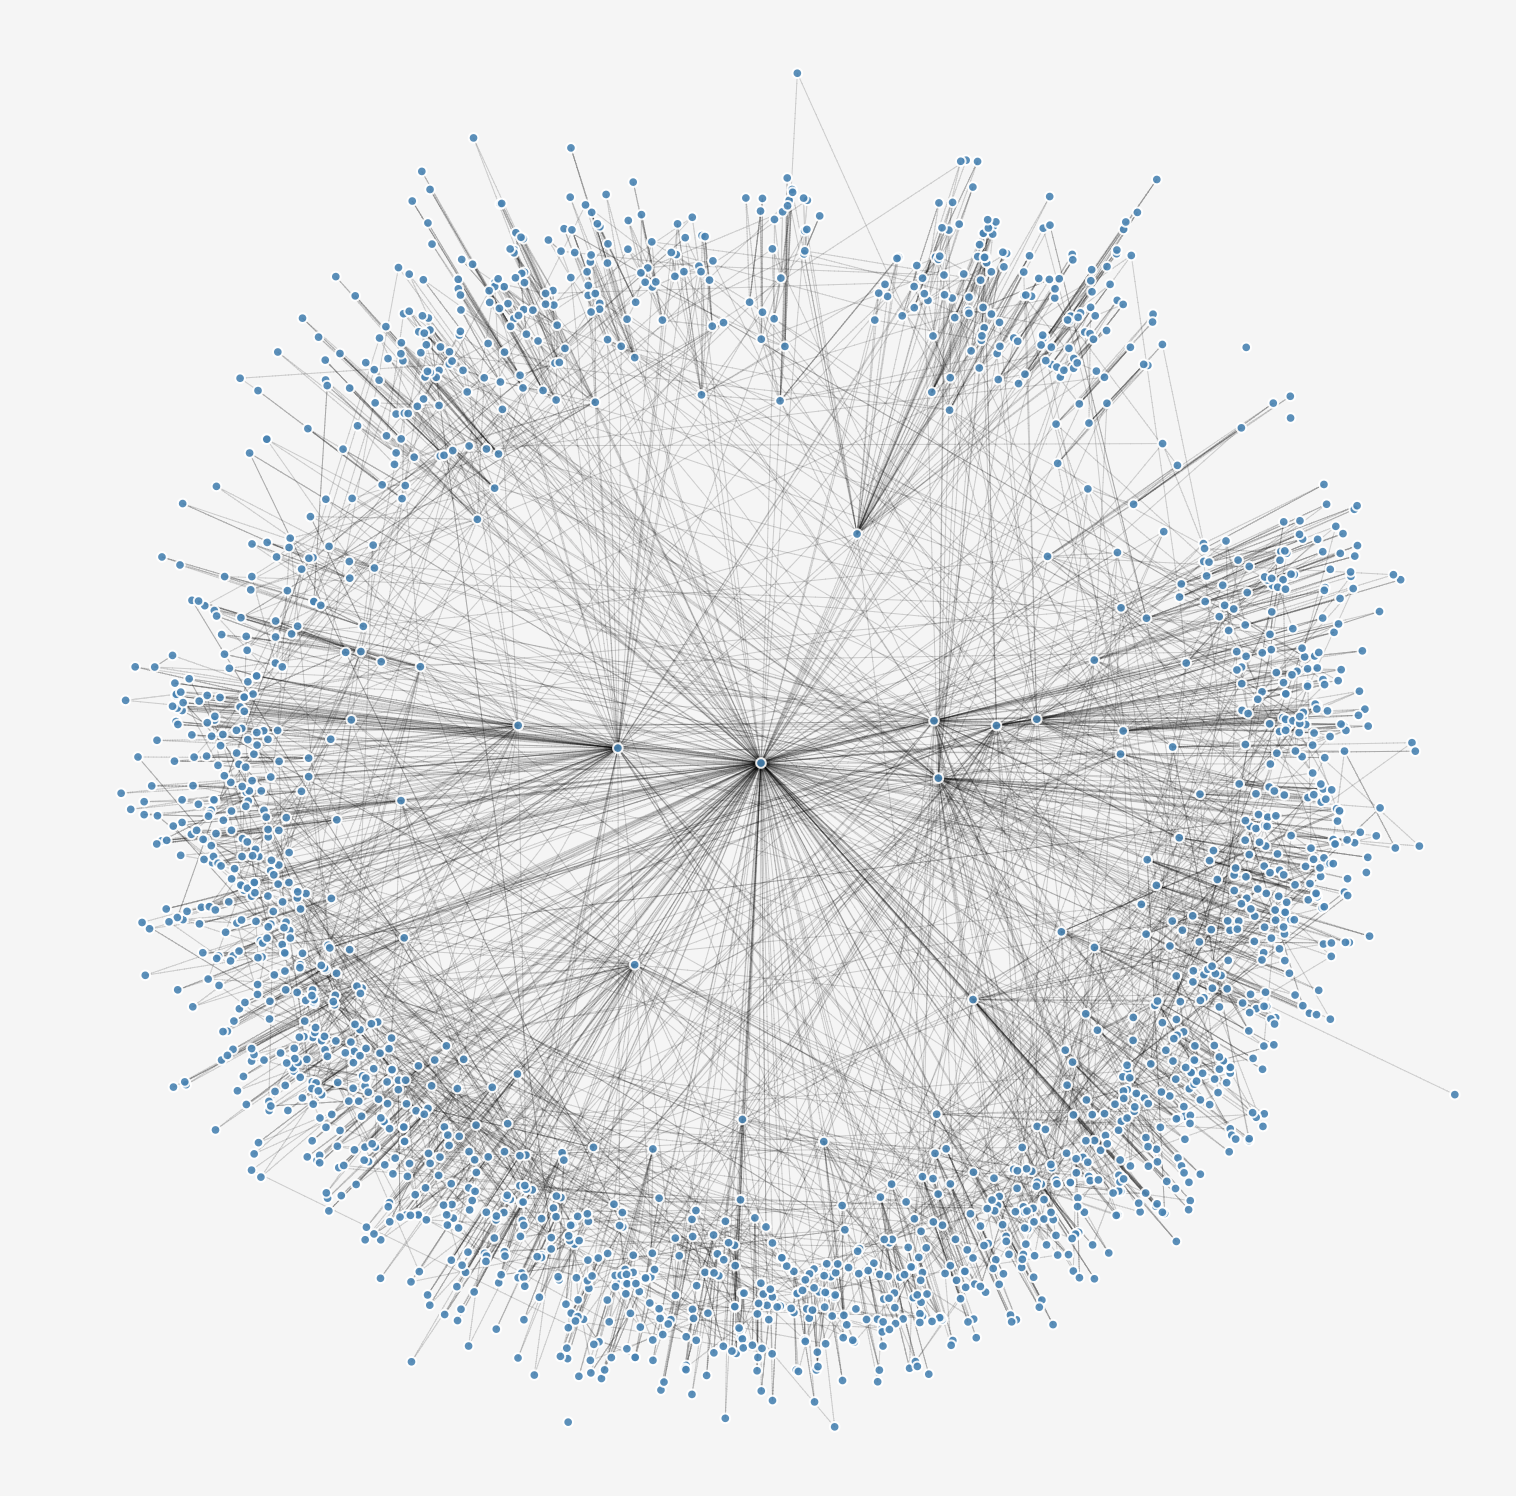
\includegraphics[width=\textwidth,angle=90]{figures_c1/layout/merc1.png}
         \caption{The Mercator graph.}
     \end{subfigure}
    \begin{subfigure}[b]{.495\textwidth}
         \centering
     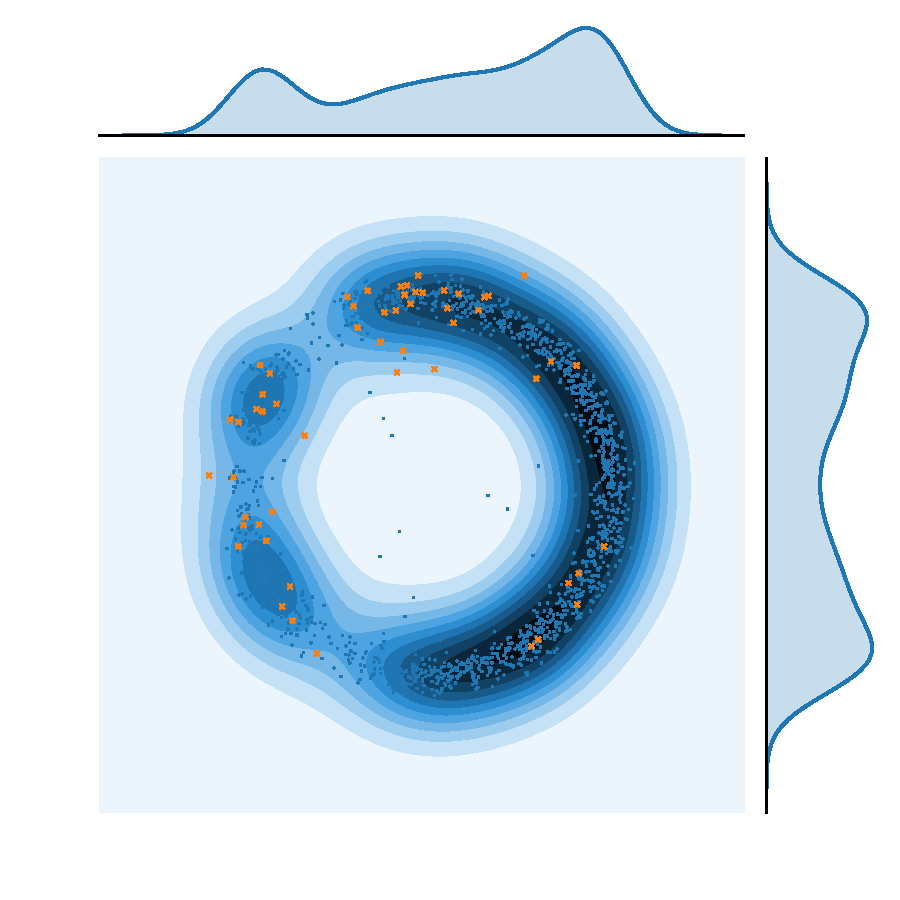
\includegraphics[width=\textwidth]{figures_c1/layout/merc_aphh.pdf}
     \caption{Mercator species distribution}
     \end{subfigure}
        \caption{\textbf{The Mercator Projection.} (a) represents output from the mercator graph layout algorithm. (b) provides a kernel density analysis of the node distribution within this. }
        \label{fig:merc}
\end{figure}

\subsubsection{Force-Directed}

Force directed graph layouts are the results of the Spring-Electrical model. This was first introduced by \cite{Eades}, and further improved by \cite{raingold}. Force-directed layouts are in essence a simple physics simulation of of like-charged particles (or nodes). These particles are repulsed by eachother, much like protons experiencing Coulomb repulsion, and try to get as far away from each other. Should a relationship exist between two nodes, we introduce an attractive force between them. These attractive forces act much like springs drawing the nodes back together. 

In the case of a weighted graph (where each link (or relationship) has a value associated with it, we can adjust the spring coefficient of the attractive force to reflect this. This results in a layout where strongly connected objects are drawn together, and weakly connected ones further away. Uses for this type of representation have been seen biology, social networks, and with this thesis atmospheric chemistry \cite{ch3,ch4}.



\paragraph*{Barnes Hut Algorithm}
Since calculating the attractive/repulsive forces for each node of a large graph can be computationally intensive, many force directed layouts rely on the Barnes-Hut approximation.

This solves the N-body problem of pairwise reactions between nodes, $O(n^2)$, by approximating long-range reactions by grouping such nodes and applying a single action on their centre of mass- reducing the computational time to $n \log n$.  

To do this, first a spatial index of each node is constructed (see below). This can either be done using a quadtree (2D) or octree (3D) algorithm. Next the centres of mass are calculated, and finally the repulsive forces for the graph are approximated. 

\textbf{Quadtree Construction:}
A quadtree is the recursive partitioning of two dimensional space into a set of quadrants (a set of 4 squares). This process is repeated, with each square then being divided into 4 itself, until there is only a single point within a cell\footnote{See \autoref{fig:quadtile} for a complete evolution of the methane quadtree.}. This converts a network, into a hierarchical tree representation of the nested quadrants in which each point resides (a quadtree), \autoref{fig:quadgroup}. 


\begin{figure}[H]
 \centering
    \begin{subfigure}[b]{.3\textwidth}
  \centering 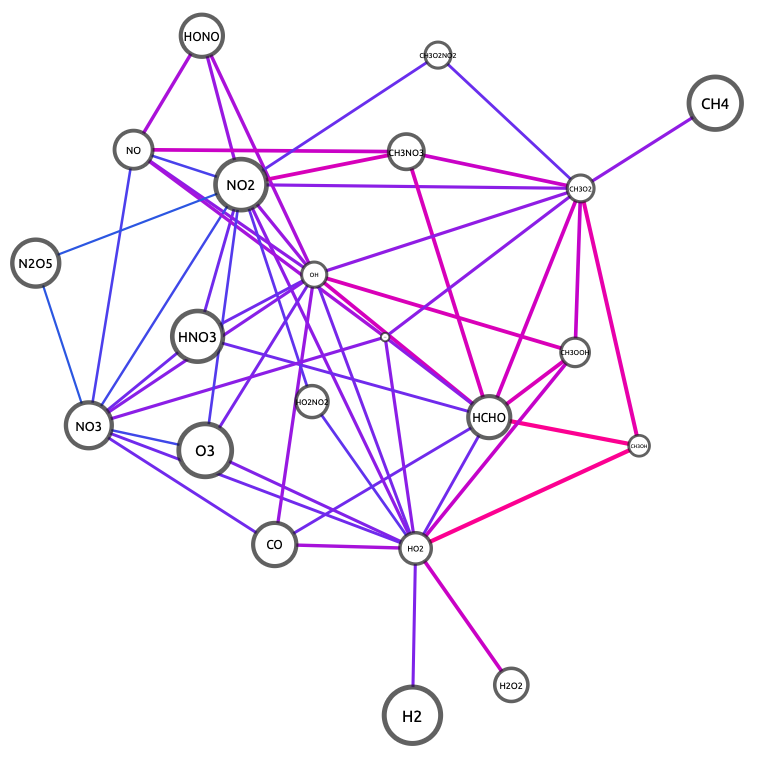
\includegraphics[width=\textwidth]{figures_c1/layout/methanequad.png}   
  \caption{Ethane Graph} 
  \label{fig:quadmeth}
 \end{subfigure}
 \begin{subfigure}[b]{.6\textwidth}
  \centering 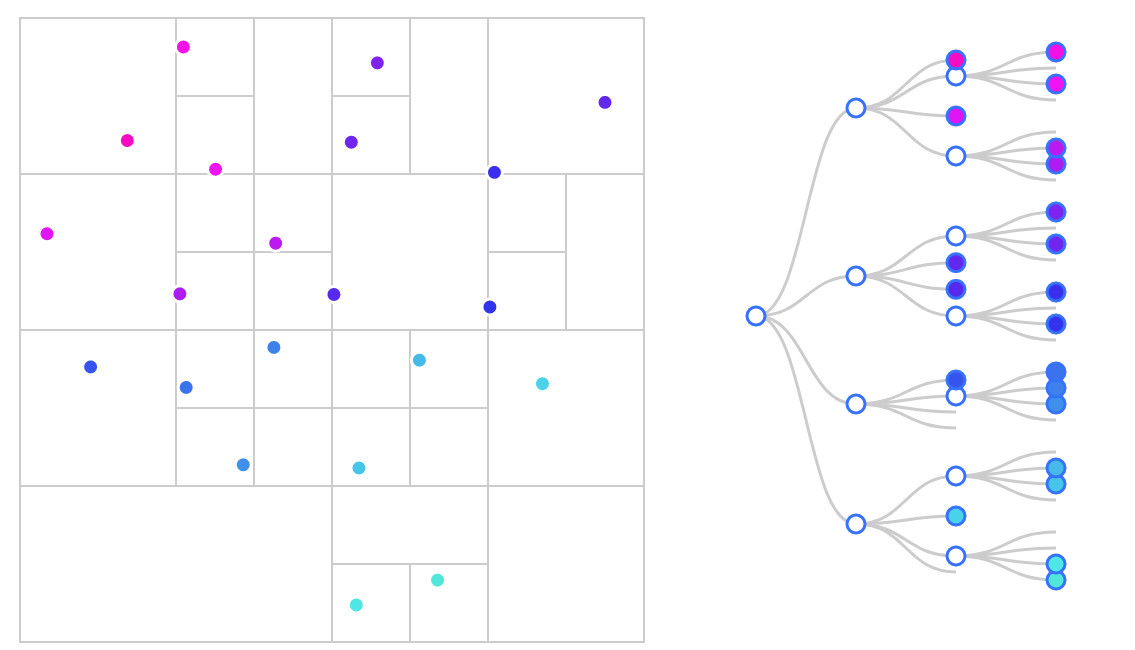
\includegraphics[width=\textwidth]{figures_c1/layout/quad.png}
 \caption{Quadtree constructed from \autoref{fig:quadmeth}}
\label{fig:quadtree}
\end{subfigure}
\caption{ \textbf{Demonstration of the formation for a quadtree from a force directed graph of Methane (including inorganics)}. (a) shows the force directed graph, (b) is the quadtree that has been constructed from this starting with the top left corner and (c) is the hierarchical tree layout of how each nodes classification based on the quadtree. }
\label{fig:quadgroup}
\end{figure}

\paragraph{Force Atlas 2}
The force atlas 2 \cite{fa} algorithm is a force directed layout designed primarily for scale-free\footnote{Definition in next chapter.} network spatilisation. It is primarily designed for the use of networks consisting of 10 to 10,000 nodes and uses barns-hut approximation for the calculation of forces. Attractive forces are derived from the spring-electric model, and follow the trend of $F_a = -k.d$, where k is the spring constant and d is the distance between the two nodes. Optional features for the graph include dissuasion by degree (separating nodes with a high number of total links/reactions), logarithmic attraction forces, adjustable gravity (attraction the centre of mass of the system to prevent disconnected components from drifting away) and collision detection to prevent overlapping nodes. 

\paragraph{Yifan Hu}
The Yifan Hu graph layout, \cite{yh}, is a multi-level graph drawing algorithm which uses the barnes-hut algorithm with an octree layout. As with the force atlas algorith, Yifan Hu also has an adaptive cooling aspect to it. This means that as the algorithm is run, its energy is progressively reduced, allowing the system to settle within a low energy state.  

The main difference within the algorithm however is the use of the multilevel approach. This has been applied to graph partitioning [11,12,23], matric ordering [24] and the travelling salesman problem [5]. This works by graph coarsening (coalescing neighbouring nodes and weighting them), running the algorithm on the course graph, prolongation and then refining the results. This produces an algorithm that runs faster than the Force Atlas, however is constrained to only working on un-directed edges.

% [10] G. Karypis and V. Kumar, “Multilevel k-way Partitioning Scheme for Irregular Graphs,”
% Journal of Parallel and Distributed Computing, 48(1), 1998 pp. 96–129.
% [11] B. Hendrickson and R. Leland, “A Multilevel Algorithm for Partitioning Graphs,”
% Technical Report SAND93-1301, Albuquerque, NM: Sandia National Laboratories,
% 1993. Also in Proceeding of Supercomputing’95 (SC95), San Diego, CA
% www.supercomp.org/sc95/proceedings/509_BHEN/SC95.HTM.
% [12] C. Walshaw, M. Cross, and M. G. Everett, “Parallel Dynamic Graph Partitioning for
% Adaptive Unstructured Meshes,” Journal of Parallel and Distributed Computing, 47(2),
% 1997 pp. 102–108.
% [13] D. Harel and Y. Koren, “A Fast Multi-Scale Method for Drawing Large Graphs,” Journal
% of Graph Algorithms and Applications, 6(3), 2002 pp. 179–202.
% [14] R. Hadany and D. Harel, “A Multi-Scale Algorithm for Drawing Graphs Nicely,”
% Discrete Applied Mathematics, 113(1), 2001 pp. 3–21.
% 70 Yifan Hu
% The Mathematica Journal 10:1 © 2006 Wolfram Media, Inc.
% [15] P. Gajer, M. T. Goodrich, and S. G. Kobourov, “A Fast Multi-Dimensional Algorithm for
% Drawing Large Graphs,” Lecture Notes in Computer Science, 1984, New York:
% Springer-Verlag, 2000 pp. 211–221.
% [16] D. Tunkelang, “A Numerical Optimization Approach to General Graph Drawing,”
% Ph.D. thesis, School of Computer Science, Carnegie Mellon University, Pittsburgh, PA,
% 1999.
% [17] A. Quigley and P. Eades, “Fade: Graph Drawing, Clustering, and Visual Abstraction,”
% Lecture Notes in Computer Science, 1984, New York: Springer-Verlag, 2000
% pp. 183–196.
% [18] A. Quigley, “Large Scale Relational Information Visualization, Clustering, and Abstraction,” Ph.D. thesis, Department of Computer Science and Software Engineering,
% University of Newcastle, Australia, 2001.
% [19] R. Davison and D. Harel, “Drawing Graphs Nicely Using Simulated Annealing,” ACM
% Transactions on Graphics, 15(4), 1996 pp. 301–331.
% [20] R. Fletcher, Practical Methods of Optimization, 2nd ed., New York: John Wiley & Sons,
% 2000.
% [21] K. J. Pulo, “Recursive Space Decompositions in Force-Directed Graph Drawing Algorithms,” in Proceedings of the Australian Symposium on Information Visualisation
% (InVis.au 2001), Sydney, Australia (P. Eades and T. Pattison, eds.), Conferences in
% Research and Practice in Information Technology Series, 9, Darlinghurst, Australia:
% Australian Computer Society, 2001 pp. 95–102.
% [22] S. Pfalzner and P. Gibbon, Many-Body Tree Methods in Physics, New York: Cambridge
% University Press, 1996.
% [23] A. Gupta, G. Karypis, and V. Kumar, “Highly Scalable Parallel Algorithms for Sparse
% Matrix Factorization,” IEEE Transactions on Parallel and Distributed Systems, 8(5), 1997
% pp. 502–520.
% [24] Y. F. Hu and J. A. Scott, “A Multilevel Algorithm for Wavefront Reduction,” SIAM
% Journal on Scientific Computing, 23(4), 2001 pp.1352–1375.
% [25] C. Walshaw, “A Multilevel Approach to the Travelling Salesman Problem,” Operations
% Research, 50(5), 2002 pp. 862–877. 

\paragraph{OpenOrd}



INSERT SOMETHING HERE 


\paragraph*{Simulated Annealing}
Most iterative layouts are updated interactively from some initial configuration. In most cases this results in a minimum configuration however this is generally a local minimum rather than the desired global minimum \cite{nicelyanneal}. To overcome this the work of \cite{metropolis}, which was later formulated in general terms by \cite{kirkpatrick} was used to lay the foundation for simulated annealing algorithms.

Annealing is usually used to describe the slow cooling applied to liquids for them to reach a crystalline (totally ordered, minimum energy) form. Relating this to the spring-electrical model, it can be seen that if the atoms(nodes) are cooled too rapidly, they will from amorphous structures representing the local minima, as opposed to the desired global one.  If cooled slowly, our graph is allowed to find a thermal equilibrium at every temperature. Working from this idea, a slow cooling constant is applied, whilst occasionally supplying the system with short bursts of energy, that may allow it to overcome local minima. 





\subsubsection{Layout Selection}

Criteria, such as ability to isolate the shortest path (in our case most reactive flux), are important in determining the usefulness of a graph. Comparing different layouts \cite{eyetrack} found 68\% of user chosen routes to reflect the shortest path between them. This is due to the force directed layout placing a greater emphasis on node positions and distance than other layouts. For comparison the same study found this to be 40\% for hierarchical layouts, and only 2\% for orthogonal ones. In this subsection I look at the use of different graph layouts, and their effect on the user readability of a graph. 


\paragraph{Node Distribution}\label{sec:nodedist}

It is known that in partitioning the screen into quartiles with equal numbers of nodes (homogeneity) greatly improves the usability of a graph and increases symmetry, \cite{ch6graphredability}. The main problem with node-link diagrams is that in represeneting complex data using an algorithmic layout can often result in regions of dense, indecipherable links, called hairballs, \cite{vislarge}. Hairballs obscure nodes and edges within a region, maiking it impossible to read. Methods such as the pruning of edges, \cite{edgeprune} can be applied to networks as a means of reducing the complexity. This may be applied post computation (syntatic representation), which results in the loss of information, or during the algorithmic approximation in the OpenOrd algorithm, to produce clearer node positioning, with the edges re-introduced at the visualisation level. 

In deciding which layout algorithm produces the best graph-node homogeneity, a kernel density approach is used to compare node distributions across 2D space in \autoref{fig:merc}b and \autoref{fig:densitycompare}. 
Here small localised areas of higher density, surrounded with sharp changes in density (shown by the contour lines) is preferabe. Such a distribution would hilight the modularity of a graph and allow for the distinction between groups of species with many reactions between them, but few in another group. Graphs with a high homogeneity can be determined through the use of $x$ and $y$ kernel density plots. Here a homogenious graph will have a uniform distribution across both axis. However as we also wish to locate regions of chemistry with a high modularity (clustering), a uniformly distributed graph would not suffice. Instead we look for a near-uniform oscillatory distribution with an equal amplitude for each peak and trough.Using these criteria the Mercator (\autoref{fig:merc}b), tsNet (\autoref{fig:ts}) and Force Atlas (\autoref{fig:fa}) score the highest, with OpenOrd and Yifan containing a gaussian-like distribution across both axis which is conducive to producing a hariball. 

Next we apply prior knowlege about the graph we are trying to visualise. Here we know that the chemistry within a mechanism is determined by the oxidation of a set of primary emitted VOCs. It therefore follows that for an ideal graph layout each primary emitted species should belong to its area of high density, and not entwined within the hairball. Immediately this notion elimiates the Yifan Hu (\autoref{fig:yfan}) and Mercator (\autoref{fig:merc}b) layouts, since these both contain a high density of primary emitted species (orange crosses) within a single dense region. Using this criterion, the tsNET graph (\autoref{fig:ts}) provides the best representation, followed by the OpenOrd and ForceAtlas layout. 


\begin{figure}[H]
     \centering
    \begin{subfigure}[b]{.49\textwidth}
         \centering 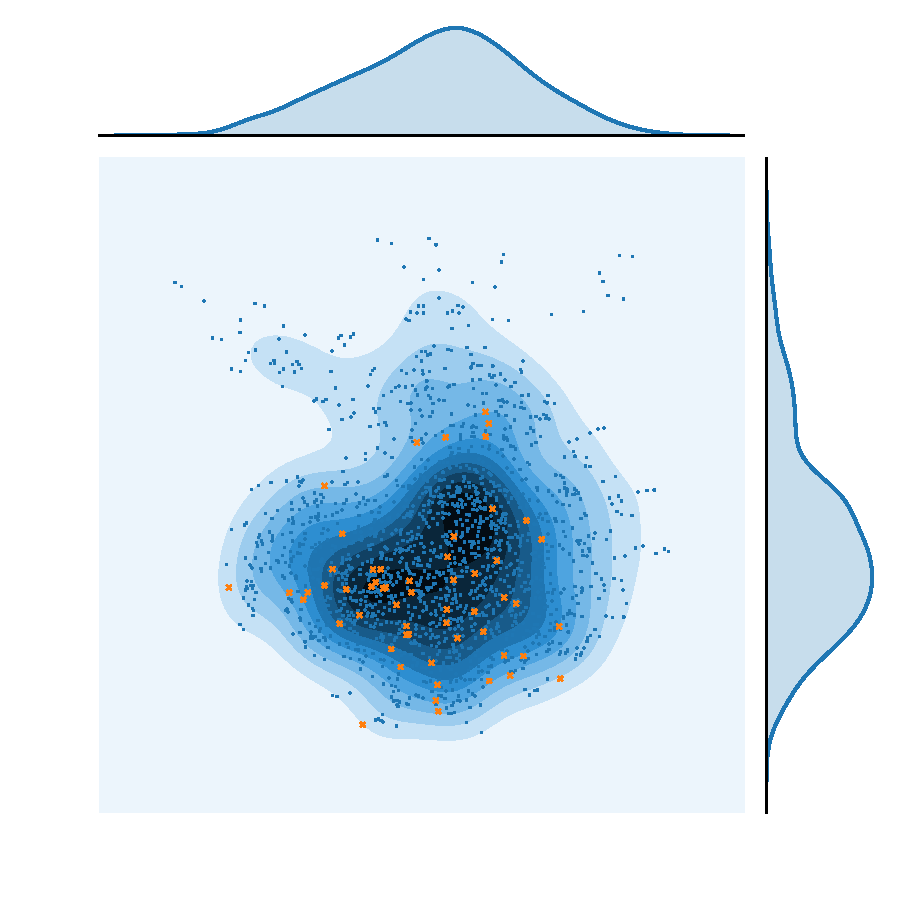
\includegraphics[width=\textwidth,angle=90]{figures_c1/layout/yfan_aphh.pdf}
         \caption{Yifan Hu}
         \label{fig:yfan}
     \end{subfigure}
     \begin{subfigure}[b]{.49\textwidth}
         \centering 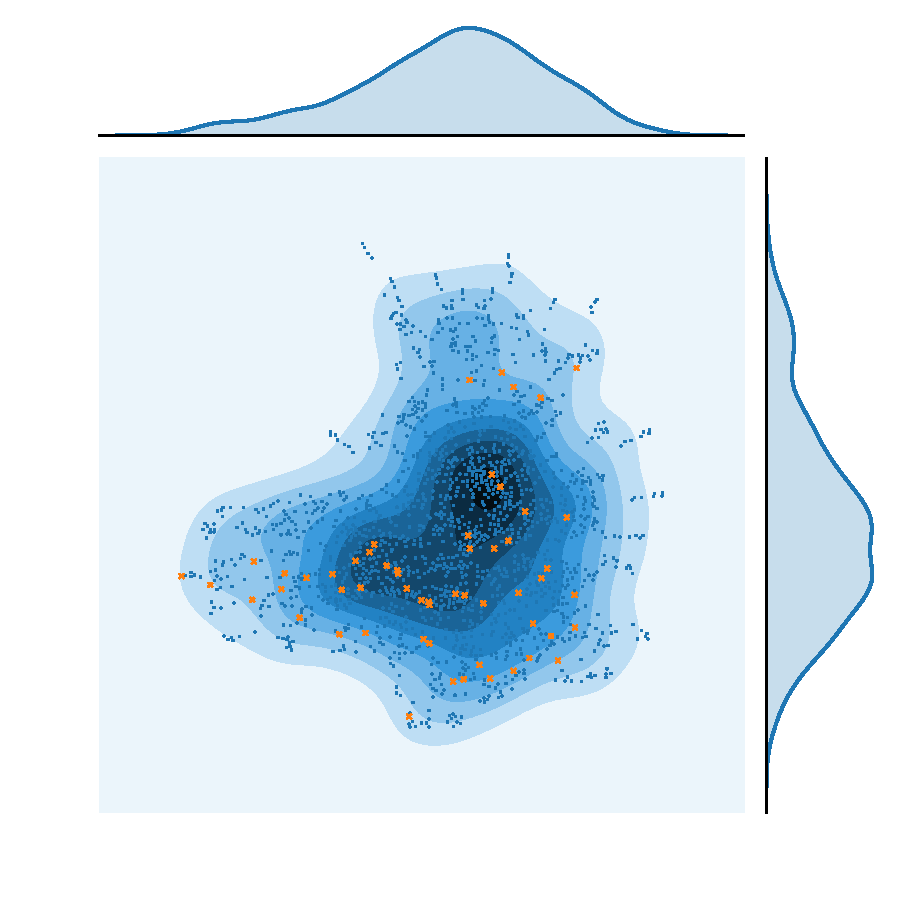
\includegraphics[width=\textwidth,angle=0]{figures_c1/layout/fa_aphh.pdf}
         \caption{Force Atlas 2}
         \label{fig:fa}
     \end{subfigure}
    \begin{subfigure}[b]{.49\textwidth}
         \centering 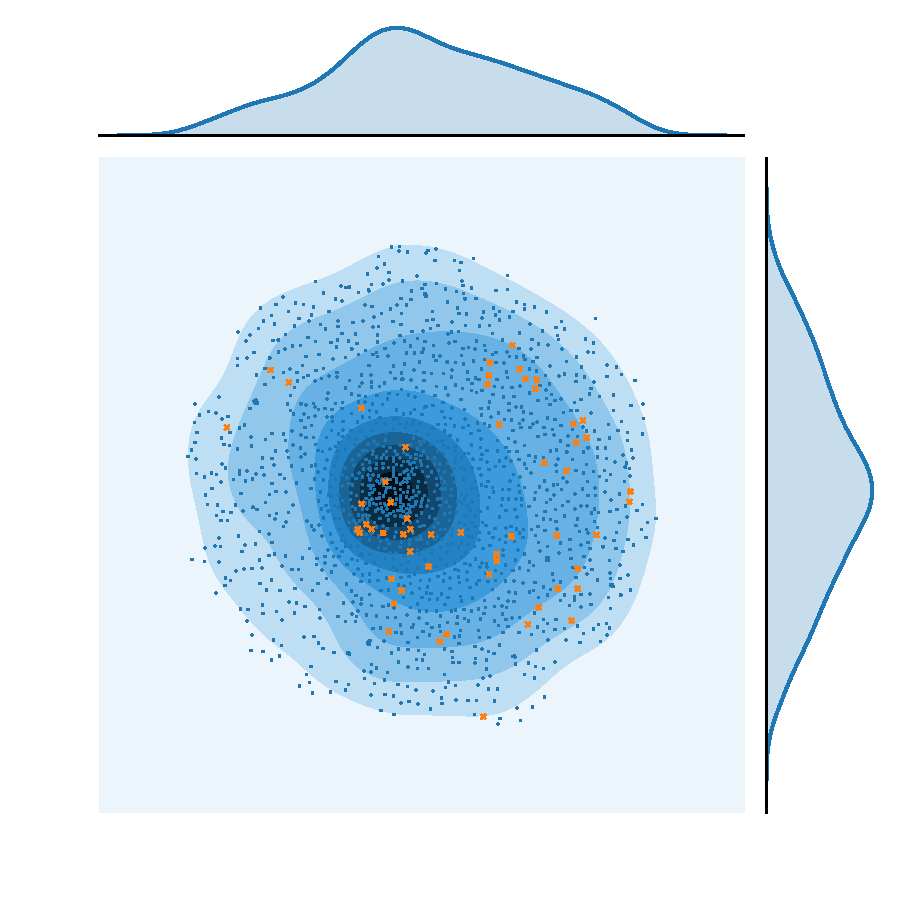
\includegraphics[width=\textwidth,angle=-180]{figures_c1/layout/oo_aphh.pdf}
         \caption{OpenOrd}
         \label{fig:oo}
     \end{subfigure}
         \begin{subfigure}[b]{.49\textwidth}
         \centering 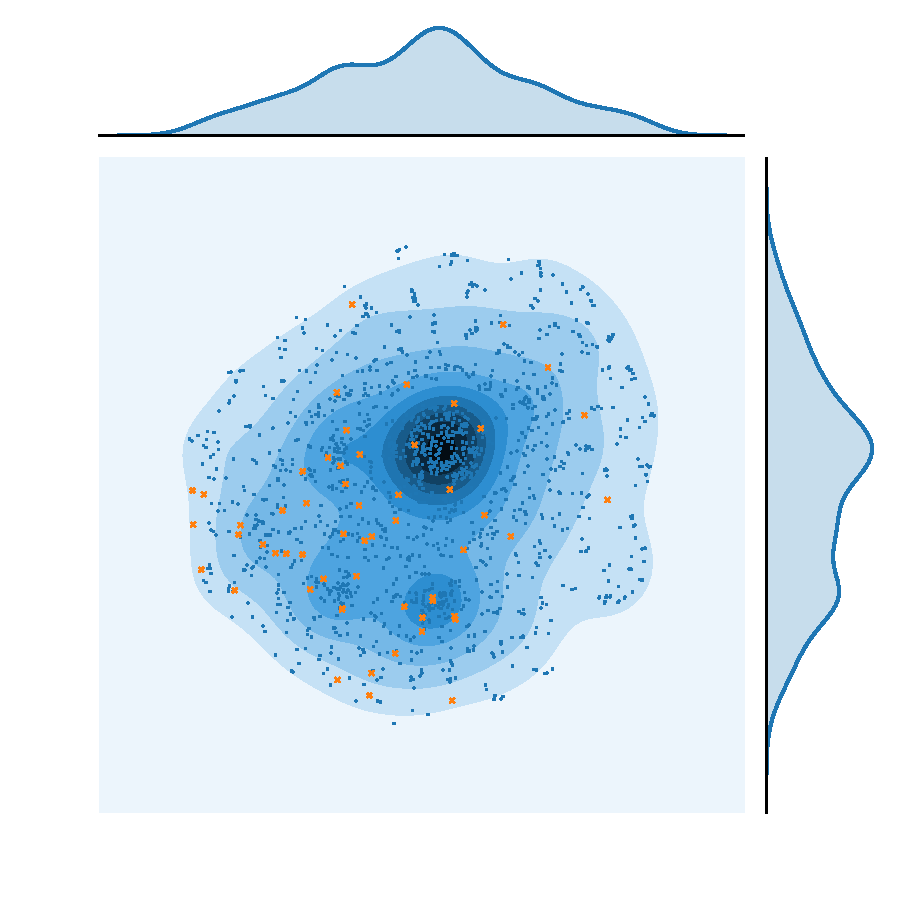
\includegraphics[width=\textwidth,angle=-90]{figures_c1/layout/tsnet_aphh.pdf}
         \caption{tsNET}
         \label{fig:ts}
     \end{subfigure}
      \hfill
        \caption{ }
        \label{fig:densitycompare}
\end{figure}




\paragraph{Node Density}
Having explored the spatial distribution of nodes within a graph, it is important to determine which layout produces the best node density variation not only across the $x$ and $y$ directions. Here we desire a degree of regular anisotropy to produce `clusters' of densely connected nodes sparsely separated in space. To calculate the distribution between dense and sparsely packed nodes, it is possible to use Voronoi tesselation. Here each node acts as a seed, and the plane is partitioned into a series of $n$ cells, where $n$ is the number of nodes. Each cell or polygon is calculated such that a polygon boundary is determined by all the points which lie closer to its source seed than any other- mathematically this would be defined as the perpendicular bisectors of the lines between all points. The result is somewhat similar to a box full of bubbles, where each bubble fills the largest area it can before meeting another. Next the area of each polygon is calculated and saved to produce a dataset representative of the complete density distribution between nodes. Here larger areas represents a species with distant neighbours (spatially), and a small one, an area of high diensity. The method of using vernouli teselation for the calculation of density has been used in the study of neurones, \cite{neurone} and areas of fixation when viewing images, \cite{fixation}. 
The last part of this process involves colouring the based on the normalised polygon area values and plotted within \autoref{fig:vornoicompare}. This allows for the easy location of layouts with high isotropy (\autoref{aoo},\autoref{ats}), which only contain many cells of a similar size, and consequently only exhibit a slight colour gradient difference between points. Although such layouts are spatially efficent, they do not reveal any additional information about the network structure. 
The colouring can also reveal the the spatial modularity of the graph. Here it is seen that the mercator, despite having a great $x-y$ node distribution, still contains large areas of unoccupied space due to its non linear density distribution. Under this criterion the ForceAtlas and YifanHu layouts (\autoref{afa},\autoref{ayfan}) perform best, with distinct modules of high density appearing to be distributed across the graph. 



\begin{figure}[H]
     \centering
    \begin{subfigure}[b]{.49\textwidth}
         \centering 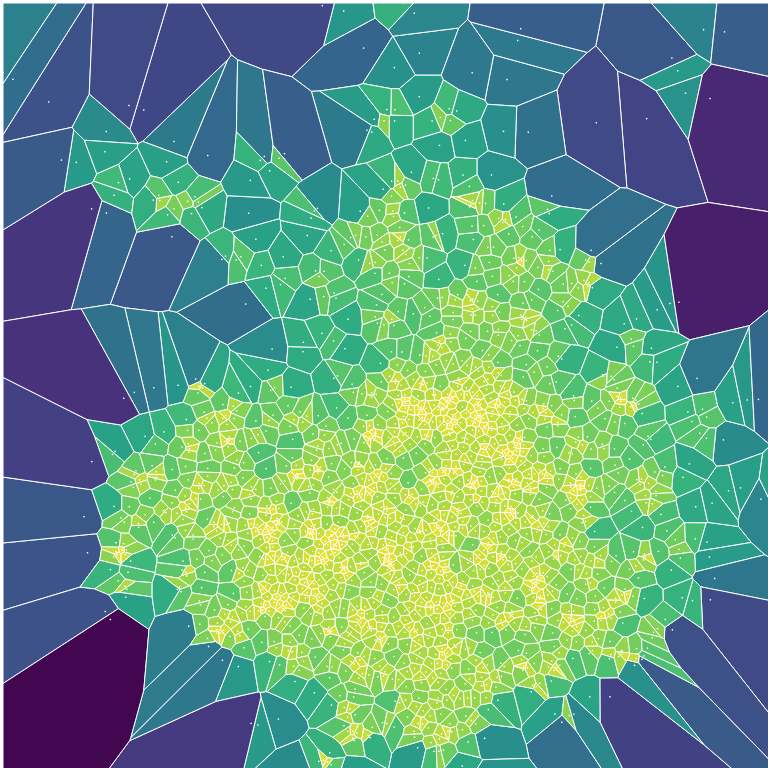
\includegraphics[width=\textwidth,angle=90]{figures_c1/area/fill_yfan_aphh.png}
         \caption{Yifan Hu}
         \label{fig:ayfan}
     \end{subfigure}
     \begin{subfigure}[b]{.49\textwidth}
         \centering 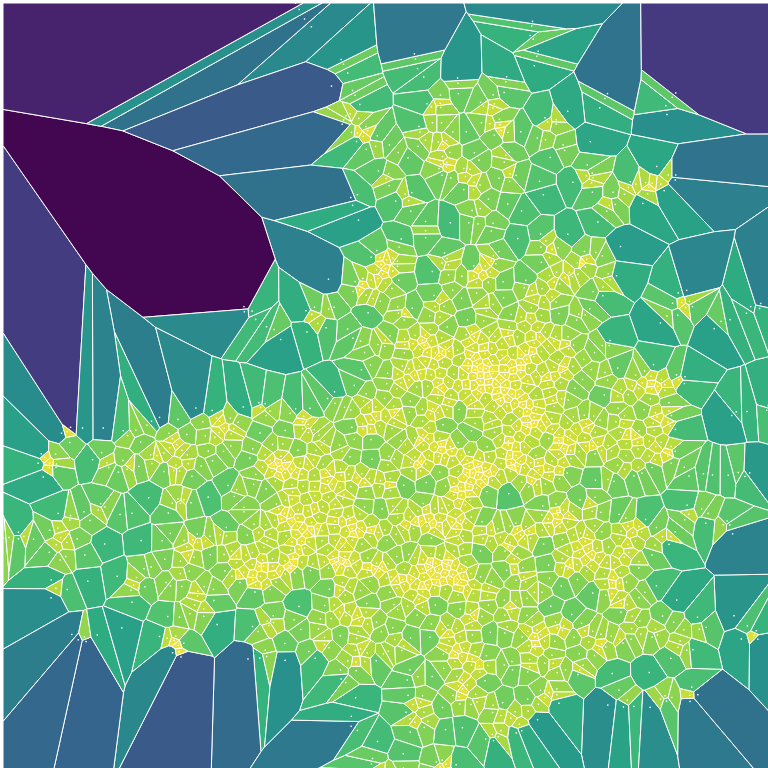
\includegraphics[width=\textwidth]{figures_c1/area/fill_fa_aphh.png}
         \caption{Force Atlas 2}
         \label{fig:afa}
     \end{subfigure}\\
         \begin{subfigure}[b]{.49\textwidth}
         \centering 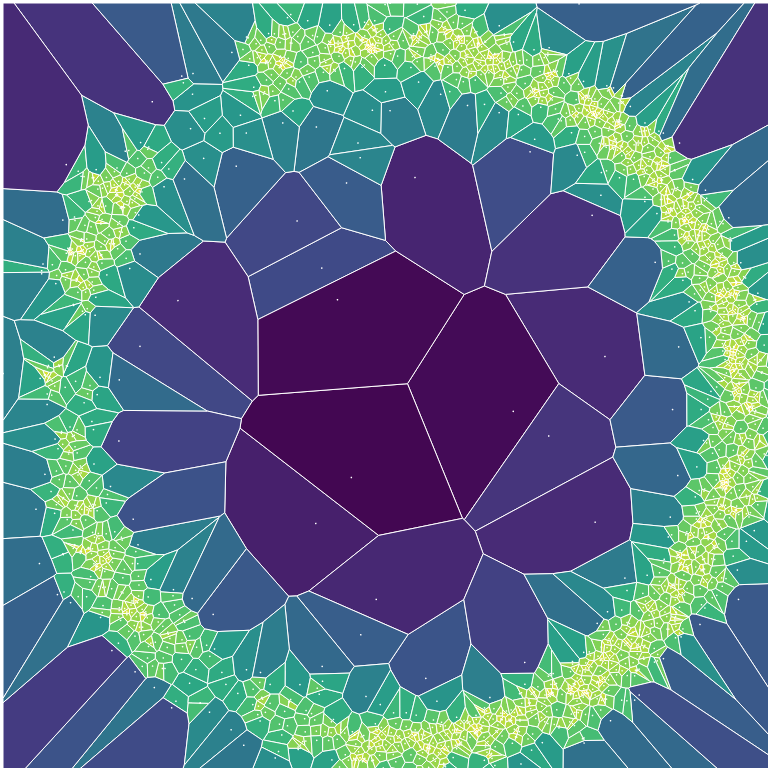
\includegraphics[width=\textwidth,angle=0]{figures_c1/area/fill_mercloc.png}
         \caption{Mercator}
         \label{fig:amer}
     \end{subfigure}
     \begin{subfigure}[b]{.49\textwidth}
         \centering 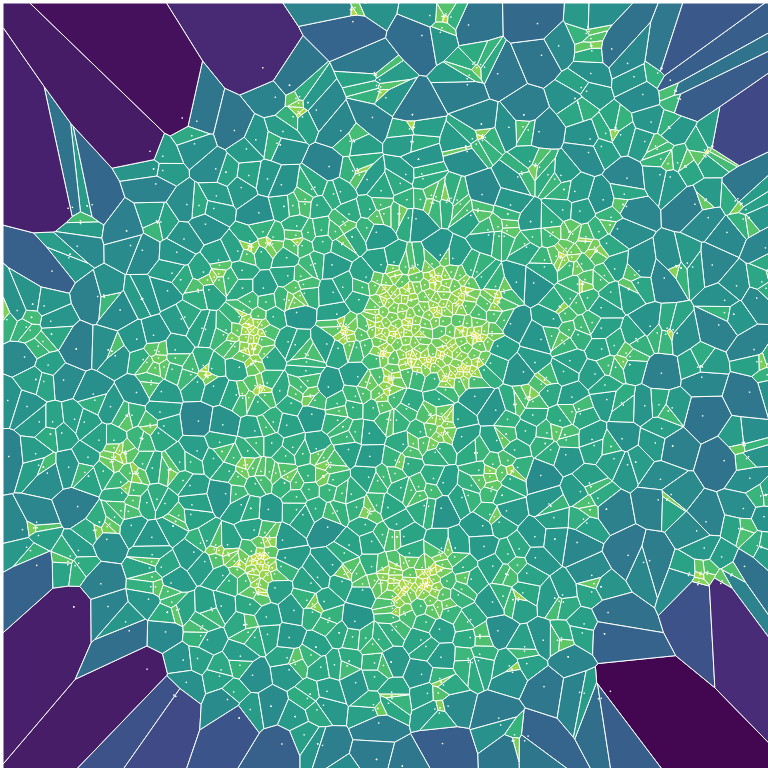
\includegraphics[width=\textwidth,angle=-90]{figures_c1/area/fill_tsnetloc.png}
         \caption{tsNet}
         \label{fig:ats}
     \end{subfigure}\\
    \begin{subfigure}[b]{.49\textwidth}
         \centering 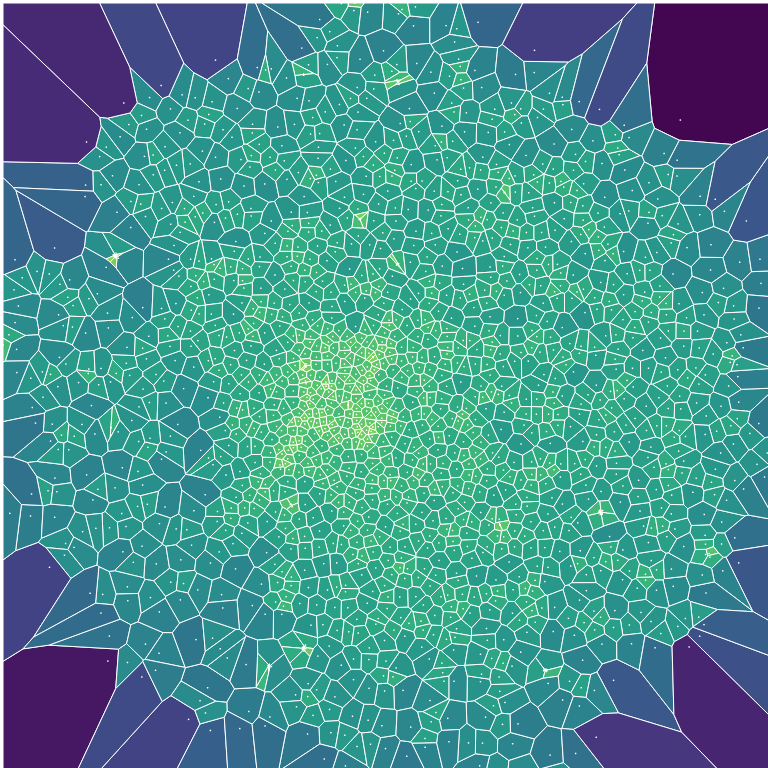
\includegraphics[width=\textwidth,angle=-180]{figures_c1/area/fill_oo_aphh.png}
         \caption{OpenOrd}
         \label{fig:aoo}
     \end{subfigure}
         \begin{subfigure}[b]{.49\textwidth}
         \centering 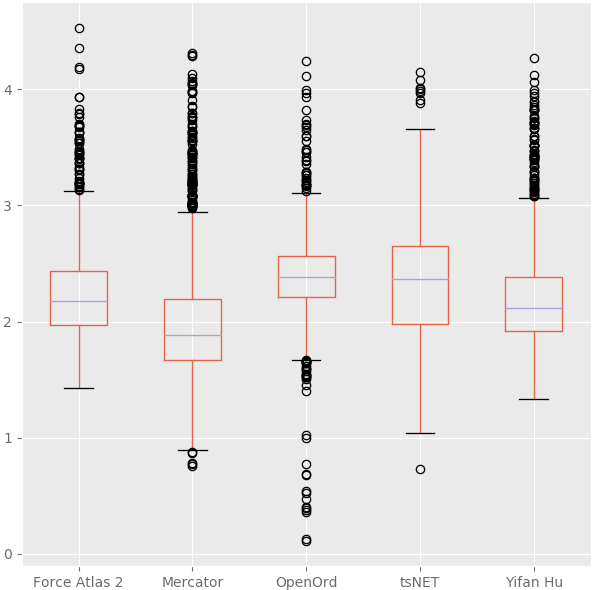
\includegraphics[width=\textwidth]{figures_c1/area/log10layoutbox.png}
         \caption{Voronoi $\log_{10}$(Area) BoxPlot}
         \label{fig:abox}
     \end{subfigure}
      \hfill
        \caption{Comparing the density of nodes for different layouts using voronoi cell areas.}
        \label{fig:vornoicompare}
\end{figure}

\paragraph{Mathematical Analysis and Layout selection}
In addition to the qualitative approach through visualisation, it is also possible represent the polygon areas for each layout in the form of several boxplots, \autoref{abox}. The interquartile (IQR) range for each layout represents the range of polygon areas. A large IQR signifies a greater distribution between low and high density  areas. 
In addition to this we are interested in having a greater ratio of smaller area polygons to larger ones. Within the boxplot, this would be represented by having a median which is closer to, or approaching the $25^{th}$ quartile ( the lower box boundary).

Applying these citerions to \autoref{abox}, shows Mercator to provide the best result. However in combining this with our previous observations, is is noted that although the ratios approach our ideal range, its radial shape is not conducive to the general represenation of modularity within a network. The layout with the largest IQR is produced using tsNET algorithm. Although this produces a well distributed algorithm, its inability to handle directed edges and high median rule it out as a possible candidate. The OpenOrd layout can reduce the number of hariballs within a graph through the use of simulated annealing and edgecutting, however it is also this property which in this case has resulted in a homogenious isotropic node distribution (as seen by the small IQR with a large median value). Unfortunately this is not seen as the most effective at hilighting the underlying structure of the chemical mechanism. 

This leaves the Force Atlas 2 and Yifan Hu layouts. Out of these the Yfan Hu layout fares better with regards to the box plot, yeilding an overall lower box, with a similar IQR and median ratio. Here its lower median suggests more high density nodes, with a similar distribution to the Force Atlas. This makes sense, since the two algorithms share many similarities, however once again the inability to handle directed edges makes it unsuitable for our application. 

This leaves the Force Atlas as the preffered layout for the visualisation of chemical mechanisms. Its directed nature coupled with intuitive design make it applicable and easy to explain, whilst still maintaining an ability to produce a clear representation of any underlying structure. In addition to this, its more uniform spatial distribution (\autoref{sec:nodedist}) makes it a better candidate than the Yifan Hu graph, which scored the highest in the boxplot test. 










